\chapter{Background}
\label{chap:background}

\section{Distributed Consensus}

% large system -° failures will occur
% somehow need to be reliable in the face of such problems
When scaling out to large number of nodes, the likelihood of a node failing increases.
Therefore, we would like the aggregate system to stay operational despite the failures of individual nodes.
A very useful primitive to reach this property is called \emph{distributed consensus}, which provides the cluster with a way to agree on a value despite individual failures.

This primitive can then be extended using asynchronous state machine replication.
In this model, the values are instructions executed by a state machine running on each node.
Since the initial state is specified, and all nodes in the cluster execute the same operations in the same order, we know that the state on every node after $i$ instruction will be the same.
Note that not all nodes might reach a given instruction at the same time.
For example, a node separated from the peers by a network failure can not receive the latest update; it will catch up later, when connectivity is restored. 
However, once a value was chosen by the cluster, we know for sure that this value will eventually be accepted by all nodes. 
In other words, it is not possible for a node to change already-made decisions. 

Typical replication protocols provide $2n + 1$ replication, meaning a cluster can stay alive as long as a majority of nodes is alive.
For example, if there are 5 nodes in the cluster, up to two could go offline without impacting the availability or the consistency of the data.
While it might seem like a good idea to make extremely large clusters, each additional node will increase the network load.
A trade off between reliability and performance must, again, be made here.

An important restriction to make is the type of node failures that we are concerned with.
We will be using the \emph{non-byzantine} model of failures\cite{paxos_made_simple}, in which the following properties hold.
First, nodes may fail by stopping, and may restart (note that this requires persistent storage in case all nodes die).
In particular, nodes are assumed to be non-malicious and non-bogus.
Messages can be re-ordered, can be duplicated, lost or delayed, but they cannot be corrupted.
Dealing with those types of failure (especially malicious nodes) require a different set of algorithms, with significantly more complexity and less performance.

\subsection{Raft Consensus Protocol}

Raft\cite{raft} is a protocol that proposes a solution to the distributed consensus problem.
Its main goal is to be easy to understand while still being efficient.
It achieves its objective by cleanly separating different concerns of the protocol.
It also provides a strong leader, \ie all entries flow from the leader to the followers, making it simpler to reason about.
Raft provides a complete solution to build a replicated state machine; the original Paxos\cite{paxos} only only provides agreement on a single value and requires an external leader election mechanism.


\begin{figure}
    \centering
    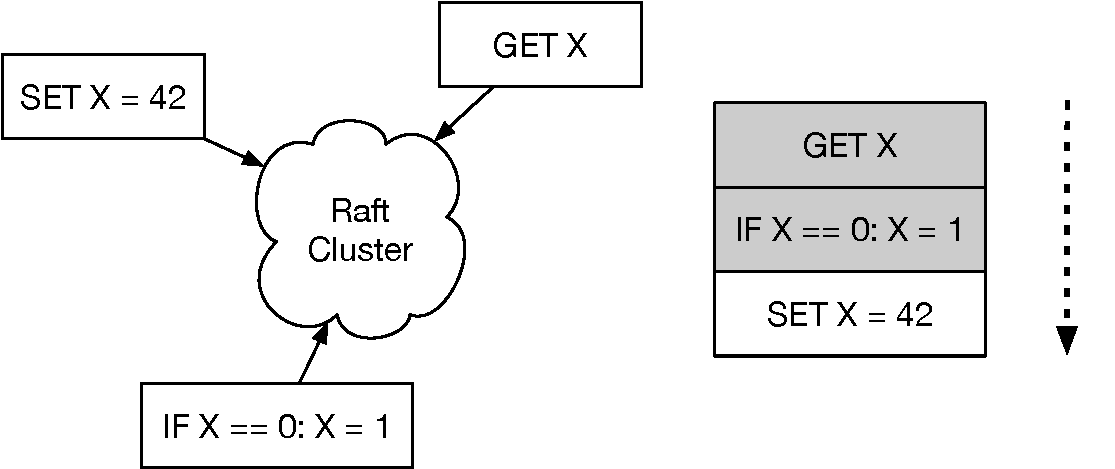
\includegraphics[width=0.8\textwidth]{replicated_log}
    \caption{Example asynchronous operations for a simple key value store supporting atomic compare and swap operation.
        Also shown on the right is the replicated log.
        Entries in grey are committed, meaning they will never be overwritten, while the last one cannot be assumed to be persistent yet.
    \label{fig:replicated-log}
    }
\end{figure}

The approach chosen by Raft to model the consensus protocol is called a \emph{distributed log}.
Under this approach, the values replicated by Raft are put inside a queue called the log (Figure~\ref{fig:replicated-log}).
Raft then replicates the log on all nodes, and guarantees that all the logs in the cluster will have the same operations in the same order.
Raft also keeps track of which entries are replicated on every node.
Once an entry has been replicated on a majority of machines, Raft guarantees it will never be removed from the log again.
Such entries are called \emph{committed}.
Raft log entries can be used as instruction to implement a replicated state machine.

Raft can be split in three different parts: leader election, log entry replication and commit propagation.
Each node can be in one of three states: \emph{follower}, \emph{candidate} or \emph{leader}.
During normal operation (when a leader emerged), a cluster contains exactly one leader and zero candidates.
To explain how the protocol works, we will start by examining the normal condition in which there is exactly one leader and it is operating properly.
We will then explain what changes during leader election.

But first, we must introduce an important Raft concept called the \emph{term}.
One term is defined as a period of time in which there is at most one leader.
This means that in order to change the leader, a new term must be changed.
Terms are identified by their term number, which always increases.
Note that not all terms have leader, for example if no leader could be elected, the term number is incremented before starting a new round of elections.

\subsection{Log Replication}

When the leader receives a request from a client, it appends it to its local log, tagging it with its index (a monotonic entry counter) and term number.
It will then periodically send \emph{AppendEntries} requests to the followers.
Each of those contains all the entries that were not yet acknowledged by the destination follower.
It also contains the term and index of the entries immediately before the first one in the request.
This allows a follower to detect any gap between its local log and the incoming entries.

The destination follower will then append the new entries contained in the \emph{AppendEntries} request to its own log.
During this step, the entries' terms and indices are used to detect inconsistencies and duplicated entries.
It then sends a reply to the leader to acknowledge that the incoming entries were correctly replicated.
It can also notify the leader of a failure to replicate, for example due to a gap in the log.

Note that the checks performed when processing \emph{AppendEntries} requests guarantee that, if two log entries on two different machines have the same index and term, then two properties must hold\cite{raft}.
First, the two entries must store the same content.
Then, all previous log entries are also matching between the two logs.
Those consistency properties allow Raft to have a simpler entry committing mechanism.

\subsection{Log Entry commit}

We say that an entry is \emph{committed} when we know for sure that this entry will never be lost by the cluster.
We also know that a committed entry will eventually be replicated to the whole cluster.
This means that to be committed, an entry must be replicated on a majority of servers.
When an entry is marked as committed, its content can be consumed by the application.

Raft does not keep track of the commit status for each individual entry.
Instead, it tracks the last committed entry; all entries before are considered committed too.

The leader keeps track of the latest acknowledged entry for each follower.
Once an entry has been replicated on a majority of machines, the leader moves its commit index to it.
The followers are then told to update their local commit status to the new index.

\subsection{Leader Election}

In Raft, leader election is based on timers.
First, a periodic timer is used by the leader to send heartbeats to followers.
Those heartbeats are \emph{AppendEntries} requests, which can be empty if there is no new request to replicate.
Every time one of those heartbeats is received, the follower resets the second timer, called the \emph{election timeout} timer.

If no messages is received from the leader, then the election timer will fire.
The follower can then then start a new leader election.
It will first increment the term, as there can be only one leader per term.
It will then transition to the candidate state and send \emph{Vote} requests to other cluster participants.

Once a node receives a \emph{Vote} request, it decides wether or not to grant its vote to the requesting candidate.
To do so, it will first check that the candidate's term is more recent than its own.
It will also check that the candidate's log is at least as complete as its own.
This ensures that the leader's log contains all committed entries.
If this was not the case, then the leader would start replacing committed entries, leading to loss of consistency.
Finally, the node sends a reply to the candidate containing the status of its vote.

If a candidate reaches majority, then it transitions to the leader role and starts sending heartbeats.
Otherwise, the election timeout will fire again, restarting the process at a new term.
To avoid conflicting elections where no majority can occur, the timeout duration is randomized, so that election will eventually succeed.
This procedure is summarized in Figure~\ref{fig:raft-leader-election}.


\begin{figure}
    \centering
    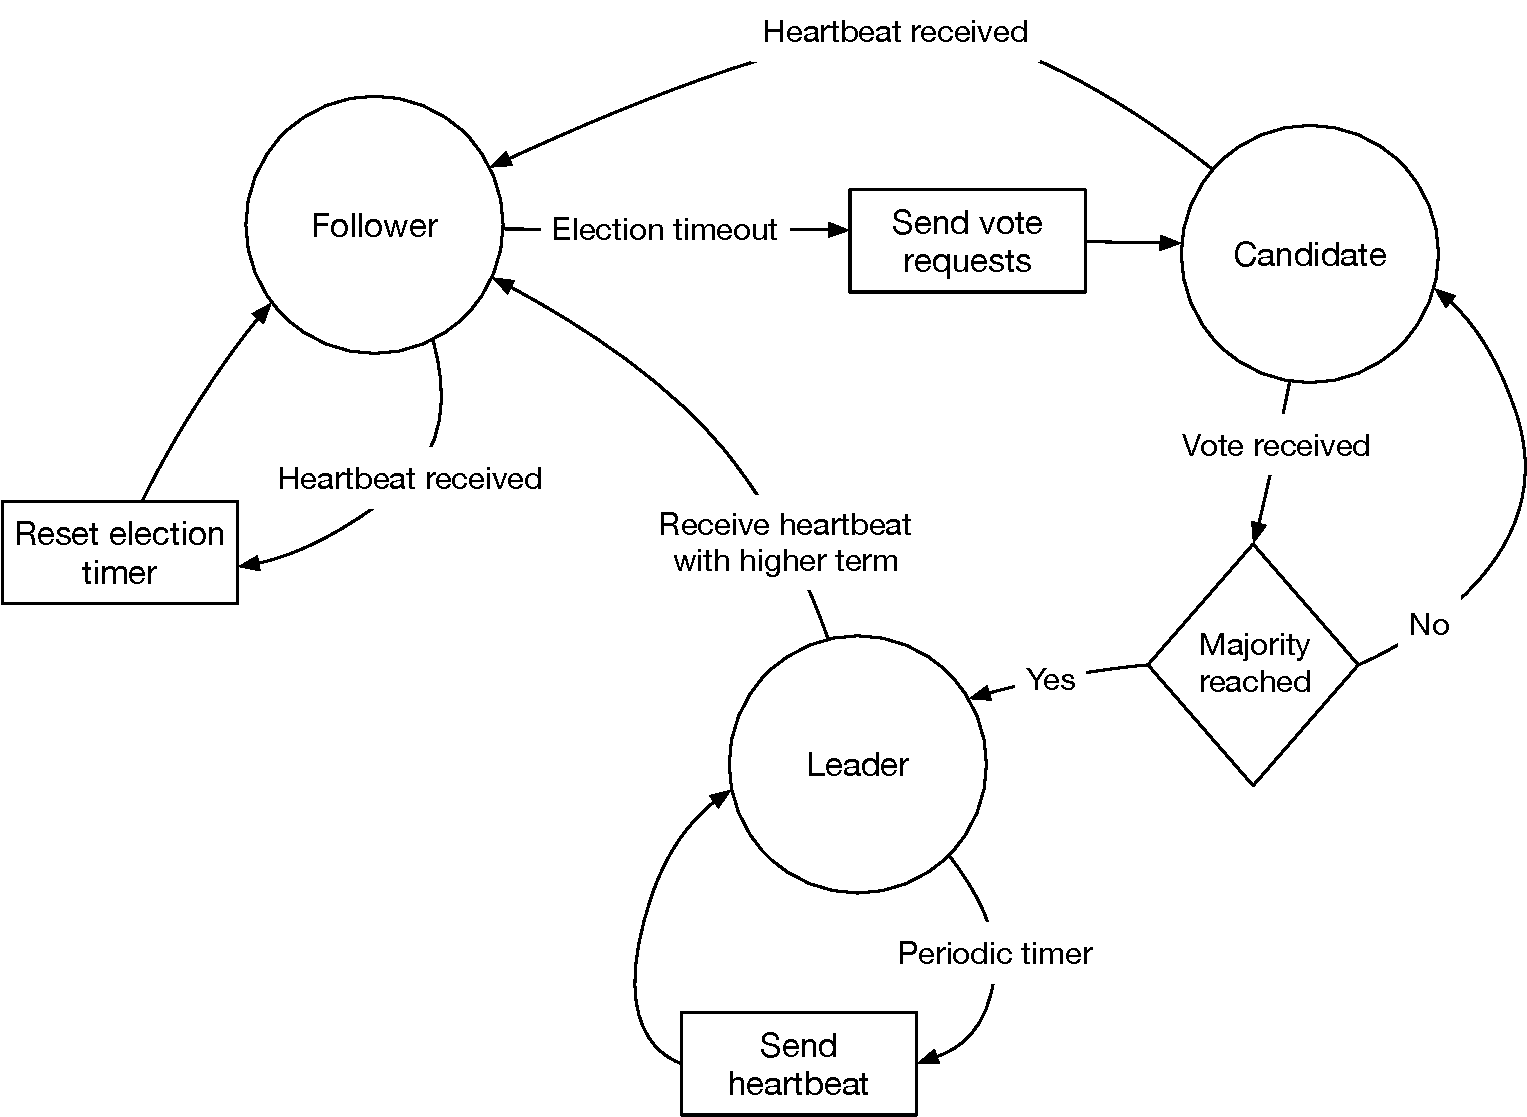
\includegraphics[width=0.8\textwidth]{raft_states.pdf}
    \caption{Raft node state machines showing leader election logic.
    \label{fig:raft-leader-election}
    }
\end{figure}


\section{Transport protocols}

% what is a transport protocol
%   Part of the internet infra
%     provides many functionalities: multiplexing, congestion control, reliable delivery, connection establishement, etc
%     handles delivery of the data to the application

Transport protocols build on the the network (IP) layer and provide services to the applications.
The most important service is multiplexing; several application can use the network, and the transport routes information to them.
This is done using port numbers.
Historically, IP was used with two transport protocols: UDP and TCP.

While UDP is very simple and only distributes incoming packets to each application (via port numbers), TCP is much more complicated.
It provides a stream interface, which guarantees that bytes that enter the connection will arrive in the same order at the other end (reliable delivery).
In order to do so, TCP has to establish a connection and then acknowledge packets.
It also provides congestion control functionality to avoid link saturation.

All those features made TCP the logical choice when sending data on the Internet, which is pretty unreliable.
However, when running inside a datacenter, packet loss or re-ordering is not as likely.
In addition to this, TCP requires multiple round trips to track connection states before being able to send application data, which increases latency (Figure~\ref{fig:tcp_lifecycle}).

%
% historical: tcp and udp
%     nowadays hard to change this due to things such as nat
%
% new protocols such as quic and
%
% need for a RPC protocol, lots used HTTP
%
% connection handshake: maybe a tcp connection establishment diagram ?


\begin{figure}
    \centering
    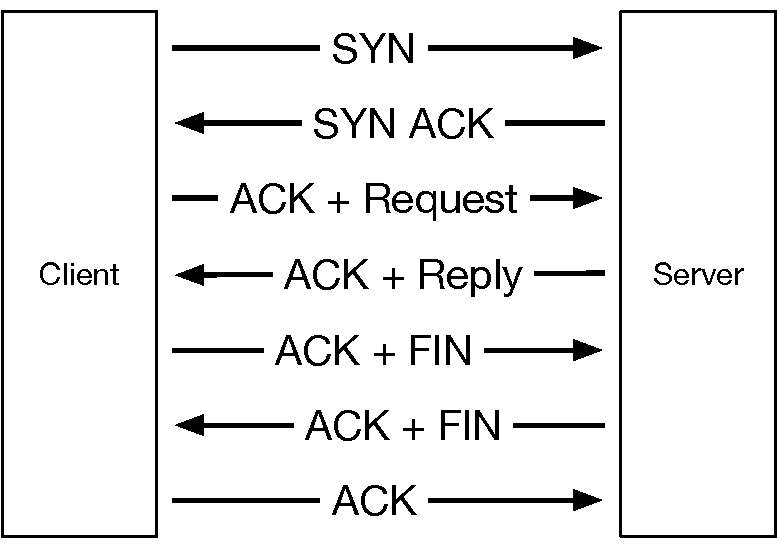
\includegraphics[width=0.4\textwidth]{tcp_lifecycle}
    \caption{Lifecycle of a typical \gls{rpc} over TCP (such as HTTP) interaction.
        We see that the latency before the reply is available takes at least two \gls{rtt}.
    \label{fig:tcp_lifecycle}
    }
\end{figure}


\subsection{Request Response Pair Protocol (R2P2)}

Most current \gls{rpc} systems, such as Google's gRPC\cite{grpc} or Facebook's Thrift\cite{thrift} typically use TCP as their transport layer.
In order to address TCP's shortcomings, the \gls{dcsl} developped a new transport protocol specially designed for \glspl{rpc}.
Unlike TCP, this new protocol is connectionless; each communication is made of a single request followed by a single response, hence the name of \glsfirst{r2p2}.
This reduces latency by removing the handshake \gls{rtt} of TCP.

\Gls{r2p2} has been succesfully used in the past to implement new load balancing techniques\cite{r2p2}.
Since it was designed with load balancing, each \gls{r2p2} request includes includes a field to specify how it should be routed.
For example, it can be marked as ``Fixed'', meaning that the request must be served by the receiver, or ``load-balanced'', in which case the router is free to redirect it to another server.
\gls{r2p2} has no notion of connections, allowing the reply to be sent directly to the client instead of having an additional trip through the load balancer (Figure~\ref{fig:load_balancing}).

\begin{figure}
    \centering
    \begin{subfigure}[t]{0.4\textwidth}
        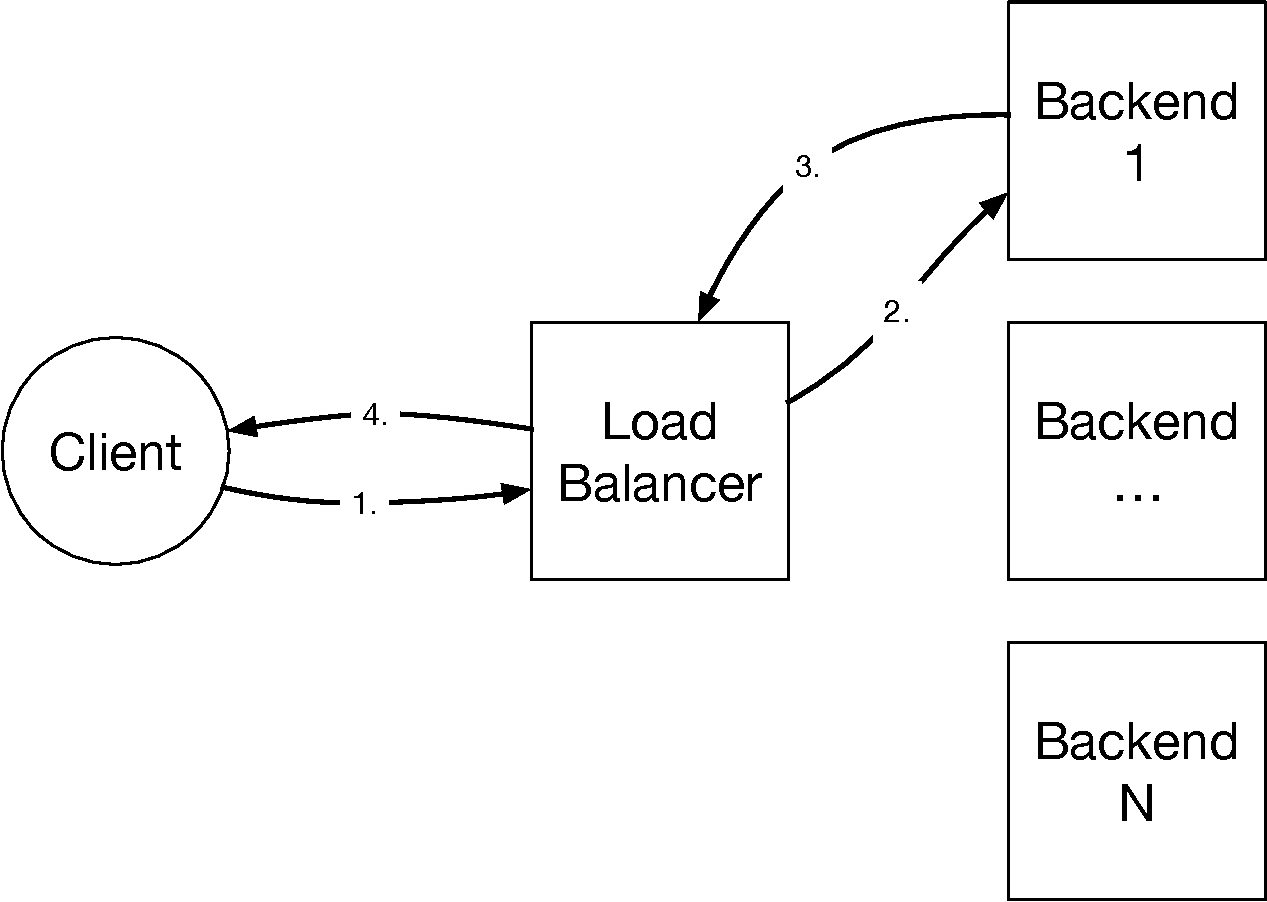
\includegraphics[width=\textwidth]{load_balancer_interaction_tcp.pdf}
        \caption{TCP}
    \end{subfigure}%
    ~
    \begin{subfigure}[t]{0.4\textwidth}
        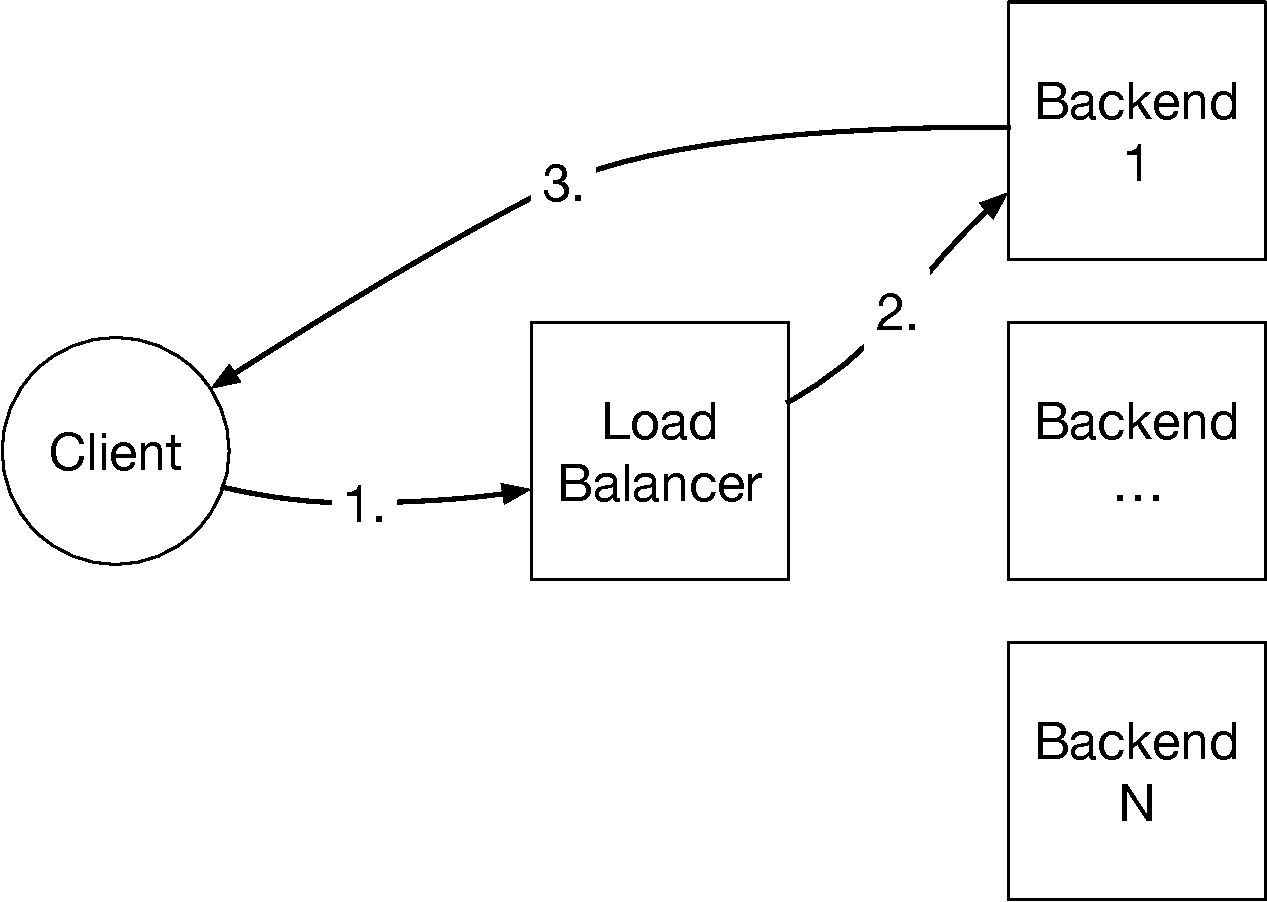
\includegraphics[width=\textwidth]{load_balancer_interaction_r2p2.pdf}
        \caption{\gls{r2p2}}
    \end{subfigure}
    \caption{
        Load balancing data flow using both TCP and \gls{r2p2}.
        We can see that the connection-less nature of \gls{r2p2} allows data to be sent directly back to the client.
        \label{fig:load_balancing}
    }
\end{figure}


We realized that it could be interesting to embed the replication mechanism in the transport layer.
This would greatly simplify the life of the application developer.
Any networked application can be turned into a replicated version of it simply by changing a flag on the requests.
Clients could even choose wether or not to ask for replication based on application-specific logic.
For example, if stales read from a key-value store are acceptable, read request could be marked as ``load-balanced'', while write requests would be marked as ``replicated'' to ensure consistency.


\subsection{R2P2 API}

The \gls{r2p2} library \gls{api} looks nothing like a BSD socket \gls{api}.
Instead it is \emph{event oriented}: the user of the library provides a set of callbacks that are called when a request is received (in the case of a server) or when a response arrives (in the case of a client).
Those callbacks also receive a per-request argument which can be used to track state.
The core of the \gls{r2p2} \gls{api} can be seen in Listing~\ref{listing:r2p2-client-api} and \ref{listing:r2p2-server-api}.

Such event-oriented \gls{api} maps well to the semantics of either high performance I/O syscalls (\eg Linux's \texttt{epoll}) or the one of kernel bypass frameworks such as DPDK.

\begin{lstfloat}
\lstinputlisting[label=listing:r2p2-client-api,caption={\gls{r2p2} client \gls{api} summary}]{code_snippets/r2p2_client_api.c}
\end{lstfloat}

\begin{lstfloat}
\lstinputlisting[label=listing:r2p2-server-api,caption={\gls{r2p2} server \gls{api}}]{code_snippets/r2p2_server_api.c}
\end{lstfloat}

With our proposal of bringing the consensus protocol to the transport layer, switching a normal application to a distributed, consistent one is simply a matter of changing the \texttt{routing\_policy} field from \texttt{FIXED\_ROUTE} to \texttt{REPLICATED\_ROUTE}.
We hope that this will create a reusable framework and that more developers will be able to write fault tolerant systems as a result.

\section{Kernel Bypass}

Due to the way time sharing operating systems work, switching between userland and kernel code, or between two userland tasks is expensive: about \SIrange{1}{2}{\micro\second}\cite{measuring_context_switch}).
This is due to the need of saving the whole original execution context first, and then loading the new execution context.
Since every system call switches to kernel code, high performance applications can be severly limited by the amount of syscall it is doing.
For example, assume that a simple packet forwarding application running on Linux uses one syscall to read a packet, and another syscall to write it again.
This means up to \SI{4}{\micro\second} of context switching per packet, restricting performance to about \SI{250}{\kilo packet\per\second}.

Another important optimization used by high performance networking code is to avoid using interrupts.
Interrupts are a way for a peripheral, such as a \gls{nic}, to notify the main processor, for example when an incoming packet is ready for processing.
They allow the processor to avoid checking the presence of processing tasks needlessly, saving computational power and energy.
However, they are also quite slow to be processed, increasing latency.
In high packet rate applications, a processor can safely assume that a packet will always be available, or just check again if this is not the case.
The loss in energy or computing power is quite low, and the gain in throughput and latency significant.
By removing context switches and interrupts, Google observed a 3x gain in throughput in their load balancers\cite{maglev}.

To reduce the number of switches between kernel space and userland, we have two choices.
The first would be to move more parts of the application in the kernel, while the second moves more parts of the system to userland.
The first option is the one that has been traditionnaly been used for networking; the TCP/IP stack or the filesystem are part of typical UNIX kernels.
This technique is very efficient in terms of developer efforts; by using the kernel-provided facilities, engineers gain access to a high-quality implementation shared by many users.
However, moving application-specific code in kernel space is not an easy task.
This is due to the usual challenges of kernel development: very little memory protection, lack of debugging tools, possibility to crash the development machine if testing on it, \etc
The lack of memory protection for kernel code also opens the door to security vulnerabilities, which can be pretty severe when processing network traffic.
While modern operating systems offer security features to mitigate this risk\cite{kernel_self_protection}, writing correct kernel code is still a difficult exercise.
This is made even more difficult by the fact that Linux's internal \gls{api} are considered unstable by developers.
This means that applications may break as kernel gets updated, making maintenance more expensive than expected.

For all these reasons, modern high performance systems tend to move more, if not all, of the stack in userland, as part of the application.
This technique is known as \emph{kernel bypass}, because it bypasses the kernel to talk to the underlying hardware directly.
In this approach, the application embeds everything it needs, from \gls{nic} drivers to TCP.
While writing a \gls{nic} driver might seem like a waste of developer's time, one generally uses framework and libraries to implement this functionality.
The main downside of kernel bypass is that it prevents sharing of ressources between applications running on the server.
For example, each networked application would need its own \gls{nic}, which can be an issue in a commercial cloud environment.
While this can be mitigated using some virtualisation techniques like SR-IOV, kernel bypass software is also more complicated to develop, and therefore reserved for performance sensitive applications.

A key contribution of our work is the use of kernel bypass techniques to reduce latency.
In particular, we are opposing our design to Kernel Paxos\cite{kernelpaxos}, which moved the Paxos consensus protocol in the Linux kernel with great results.
We believe that using kernel bypass techniques can lead to similar, if not better performance without compromising on the security benefit of process separation.
